\section{Realisation}
\subsection{Engineering work}
My work was split into many different parts. I made a \brand{GitHub} deposit : \url{https://github.com/jcelerier/spectral-subtraction} in which there are folders that correspond to these parts.
\subsubsection{Implementation of the algorithms}
This part will refer to the folder \texttt{libnoisered}. 

\paragraph{Technologies used}
As soon as I could, I tried to make the algorithms as a separate library, which has for sole dependencies \ac{FFTW} and \brand{CWTLIB++}. A corresponding \brand{Doxygen} documentation can be generated inside this folder, or by calling \texttt{make doc} on the root of the repository.

\subparagraph{Choice of \ac{FFTW}} I choose to use \ac{FFTW} because it seems that it is one of the best performing Fourier Transform, apart from implementations which are devised specially towards a particular \brand{CPU}: \url{http://www.fftw.org/speed/}.
It also supports the \brand{NEON} vectorial instructions of the \brand{ARM} processor, which can provide a performance boost.
\subparagraph{Overlap-add technique}
One of the technique used here is the overlap-add technique. Instead of performing a Fourier transform on a data-filled array, the input array is twice the data size, and its second half is filled by zeros.
After the subtraction is applied, the output array's first half is added to the previous array's last half, and so on. This is the only point on the algorithms that can't be threaded easily.
Overlap-add method can be enabled or disabled. If it is disabled, a simple rectangular window is used.
\paragraph{Spectral Subtraction}
The numerical algorithms are most of the time very straightforward.

\begin{algorithm}
 \SetAlgoLined
 \KwData{A signal spectrum X, a noise estimation Z}
 \KwResult{A new signal X' with less noise}

 \ForAll{bands $i$ in the spectrum}{
	$ t_0\gets \power(X_i)$ \\
	$ t_1 \gets t0 - \alpha * Z(i)$ \\
	$ t_2 \gets \beta * t0$ \\
	$ \mathrm{mag} \gets \sqrt{\max(t1, t2)}$ \\
	$ \mathrm{ph} \gets \phase(X_i)$ \\
	$ X_i \gets \recompute(mag, ph)$ 
	\tcp{Spectrum is given in complex format}
 }
 \caption{Simple spectral subtraction (\texttt{subtraction/simple\_ss.cpp})}
\end{algorithm}

Whenever I could, I tried to use \brand{C++ STL} algorithms, like \texttt{std::transform}, or \texttt{std::accumulate}.
There are several advantages : 
\begin{itemize}
\item They make the code very concise and readable. For instance, here is the code that computes the power for every band of a spectrum array, in complex format : 
\begin{lstlisting}[caption=math\_util.cpp]
void compute_power(fftw_complex *in, double *powoutput, unsigned int size)
{
	std::transform(in, in + size, powoutput, ToPower);
}
\end{lstlisting}

Here, \texttt{ToPower} is a \brand{C++11} lambda expression, which is used in other functions as well :
\begin{lstlisting}[caption=math\_util.cpp]
auto ToPower = [&] (fftw_complex val)
{
	return std::pow(val[0], 2) + std::pow(val[1], 2);
};
\end{lstlisting}
I choose to use a lambda-expression because common compilers seems to optimize them better than ordinary functions\cite[p.~213]{cppstl}, and here performance is critical.
\item The \brand{C++} standard imposes a maximal complexity for these algorithms. For instance, \texttt{std::max} must be in $\theta(n)$ (courtesy of \url{www.cplusplus.com}).
\item They present the advantage of having parallel versions, when using \brand{GCC}. These versions are enabled with a single \brand{G++} flag : \texttt{D\_GLIBCXX\_PARALLEL}. This way, they can be easily disabled for the embedded board, where it is inefficient because it is single-threaded, while they can be enabled when doing tests on the computer. 
\end{itemize}


\paragraph{First organisation}
At first, when there were only a few algorithms to code, it seemed logical to have a class only for noise estimation algorithms, and a class only for subtraction algorithms. However, some algorithms like the one proposed by Rainer Martin\cite{martin2001noise} uses a lot of static variables and tables, because data has to be kept from a frame to another. 
Here was the first class diagram : 
\begin{figure}[H]
\begin{center}
\hspace{-11em}
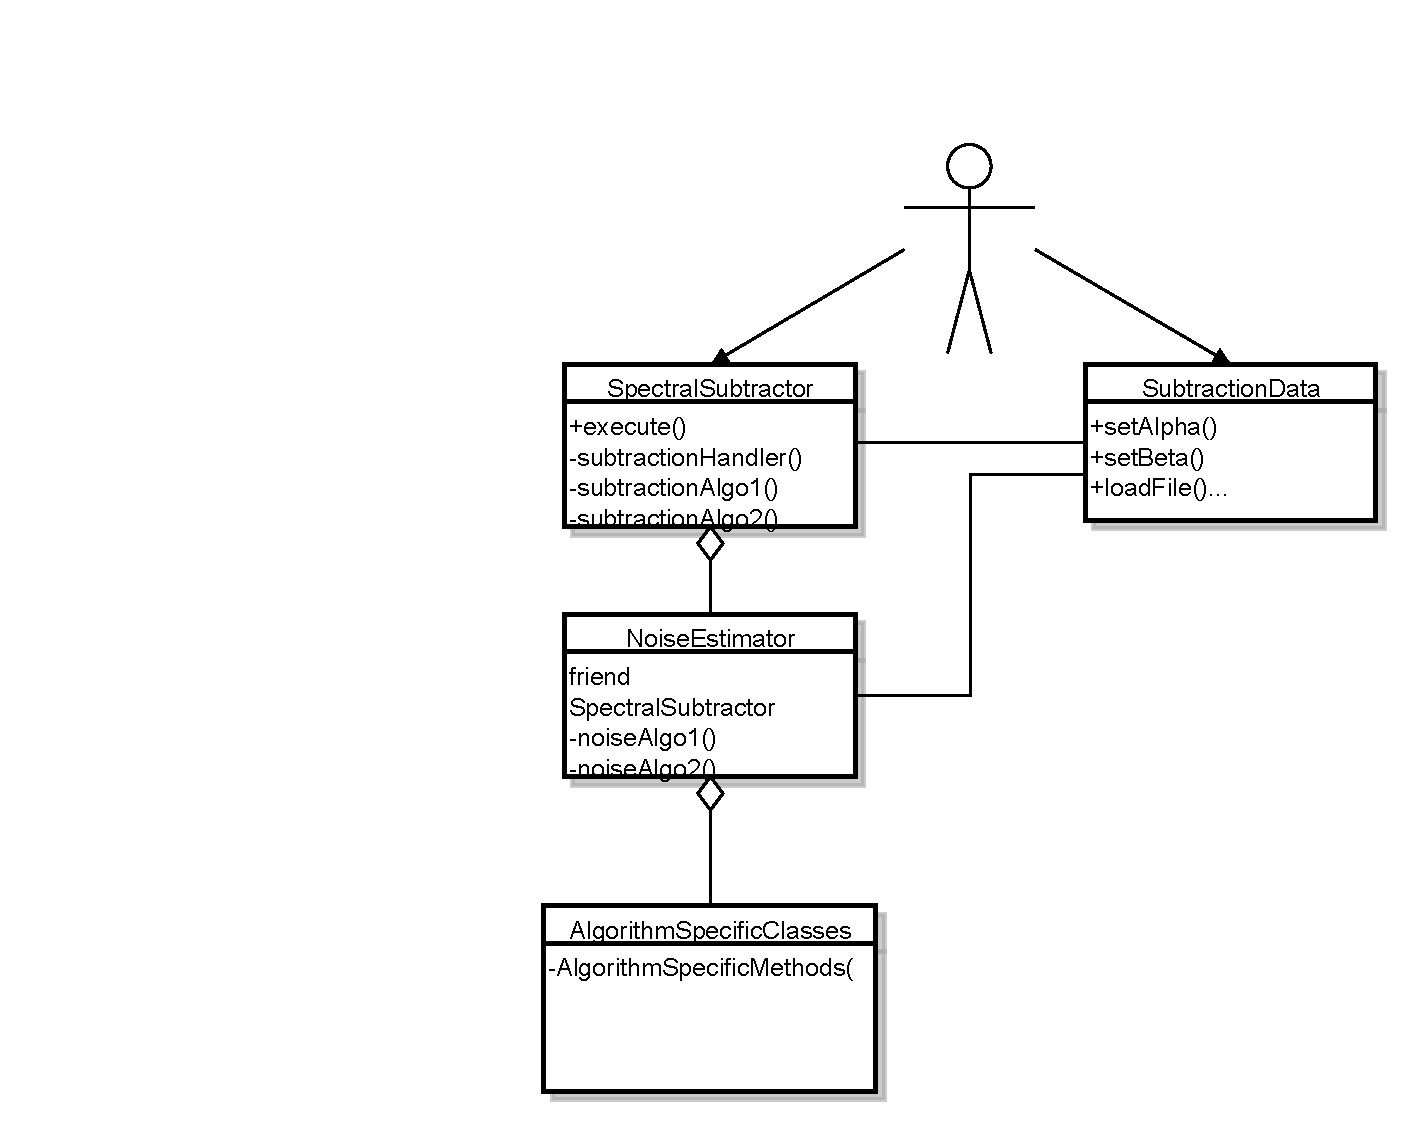
\includegraphics[scale=0.5]{old.pdf}
\caption{First organization of the library}
\label{diag_api_chords}
\end{center}
\end{figure}
The problem is that the data and the algorithms were intertwined. This could have caused problems when trying to thread. Also, the \texttt{SpectralSubtractor} and \texttt{NoiseEstimator} had to be friend with \texttt{SubtractionData}, which held many of the parameters required to perform the algorithms, like the number of iterations, etc.
Finally, the user had to manipulate two different objects, which causes unneeded clutter in the code.
\paragraph{Mid-internship reorganisation}
I then decided to refactor my code, by taking a modular approach, that would be more logical.
The user mostly interacts with the \texttt{SubtractionManager} object. This object holds : 
\begin{itemize}
\item The audio data.
\item Methods for loading an audio buffer, or a raw audio file.
\item A method to read parameters from a configuration file.
\item Methods to manage the Fourier transform.
\item Handlers to call if there is a change of data, or FFT size.
\item Methods to set general parameters, like the number of iterations, or the usage of the overlap-add method.
\item Two very important objects, of base class \texttt{Estimation} and \texttt{Subtraction}, and the associated getters and setters.
\end{itemize}
The \texttt{Estimation} and \texttt{Subtraction} objects hold the algorithm implementation. This reduces memory consumption, because only the wanted algorithm and needed implementation details are loaded, versus the previous approach where every algorithm had to be initialized. To permit a good memory management, I used a \brand{C++11} smart pointer \texttt{std::shared\_ptr} to keep them.

An example of initialization would be : 
\begin{lstlisting}[caption=Example initialization]
SubtractionManager s_mgr(fft_size, sampling_rate);
SimpleSpectralSubtraction* sub_algo = new SimpleSpectralSubtraction(s_mgr);
// Here we set algorithm-specific parameters.
// For instance they are not present in GeometricSpectralSubtraction class
sub_algo->setAlpha(data->alphaBsc); 
sub_algo->setBeta(data->betaBsc);
s_mgr.setSubtractionImplementation(std::shared_ptr<Subtraction>(sub_algo));
\end{lstlisting}

The \texttt{Estimation} and \texttt{Subtraction} objects are functors. I choose to build them with a reference to the \texttt{SubtractionManager} object because had not I done this, I would have to add at least two parameters to most methods in \texttt{Estimation} and \texttt{Subtraction}, one to get the sampling rate, and one to get the size of the arrays, because they are both needed most of the time.

\begin{figure}[h]
\begin{center}
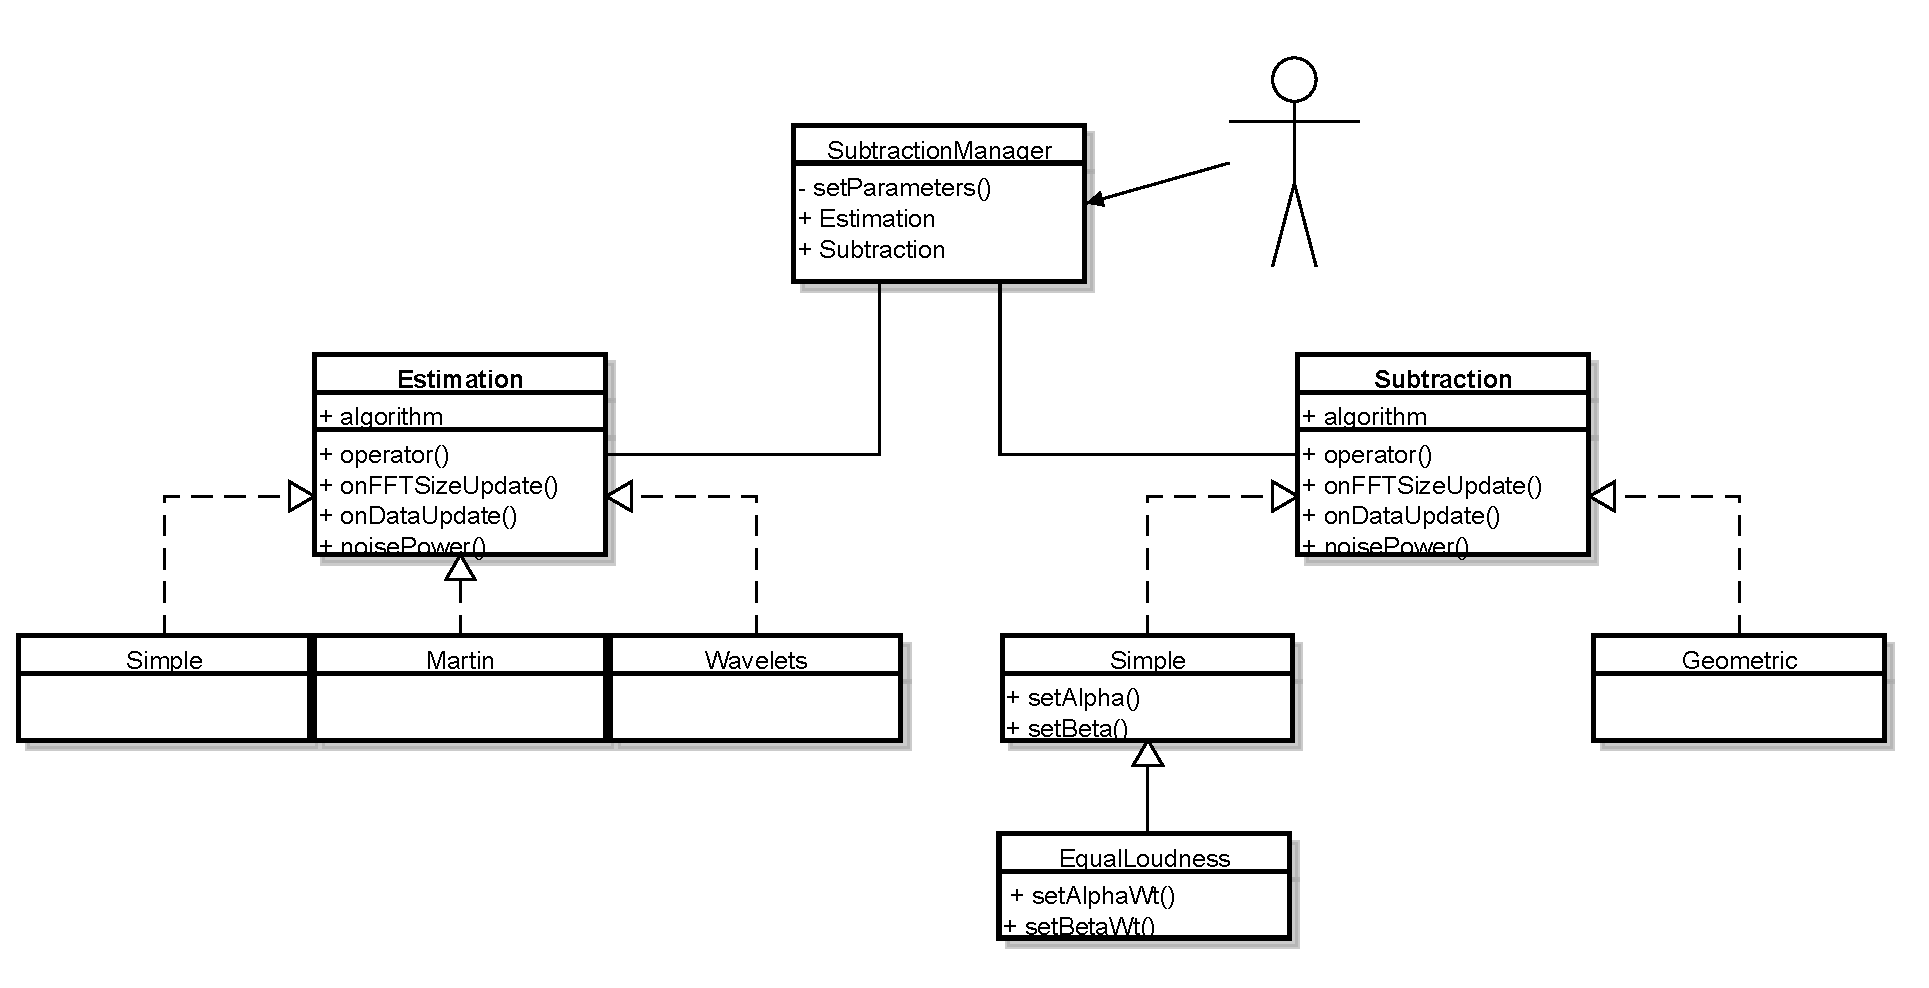
\includegraphics[scale=0.4]{base.pdf}
\caption{Current organization of the library. Not all implementation details present.}
\label{diag_api_chords}
\end{center}
\end{figure} 

The \texttt{Subtraction} class is little more than an interface, with only the constructors and destructors not being pure virtual. However, the \texttt{Estimation} class needs to keep track of the current noise estimation (in the form of an array of \texttt{doubles}). For this, I choose to use the \textbf{Template method pattern}:

Calling \texttt{Estimation::onFFTSizeUpdate()} or \texttt{Estimation::onDataUpdate()} will perform some actions needed for the noise estimation array, like resizing it, and make a subsequent call to \texttt{Estimation::specific\_onFFTSizeUpdate()} or \texttt{Estimation::specific\_onDataUpdate()}, which are left pure virtual in the base class. It is up to the real algorithms to implement them.

\paragraph{Core algorithm}
Finally, a very important algorithm is \texttt{SubtractionManager::execute()} because it is the one that gets called when the data and parameters are ready.

Thanks to the care taken in the design, the code is very short and extremely generic: 
\begin{lstlisting}[caption=\texttt{SubtractionManager::execute()} in subtraction\_manager.cpp]
for (auto iter = 0U; iter < iterations(); ++iter)
{
	for (auto sample_n = 0U; sample_n < getLength(); sample_n += getFrameIncrement())
	{
		copyInput(sample_n);
		forwardFFT();

		if(dataSource() == DataSource::File && sample_n == 0)
			onDataUpdate();

		// Noise estimation
		(*getEstimationImplementation())(spectrum());

		// Spectral subtraction
		(*getSubtractionImplementation())(spectrum(), 
			getEstimationImplementation()->noisePower());

		backwardFFT();
		copyOutput(sample_n);
	}
}
\end{lstlisting}
\subsubsection{Test application}
This part will refer to the folder \texttt{denoiseGUI}. 
\paragraph{Technologies used}
The application is fully developed using the \brand{Qt} framework, so that it can work easily on different environments (all the major desktop operating systems). It has only been tested on the \brand{Qt5} version.

\paragraph{Features of the software}
I had to make this application to compare the algorithms, and later, to perform batch processing on either a lot of files or a lot of parameters.
It can change all the relevant algorithms and parameters, load audio files and playback them before and after processing, and computes relevant evaluation parameters, the noise reduction ratio and speech distortion ratio\cite{horii2013musical}.
\begin{figure}[h]
\begin{center}
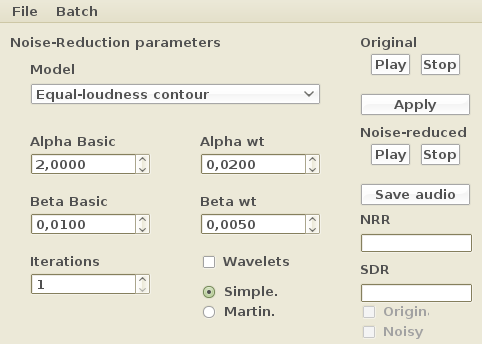
\includegraphics[scale=0.75]{testapp1.png}
\caption{Test application, upon opening}
\label{diag_api_chords}
\end{center}
\end{figure}

\subparagraph{Batch processing} It is enabled in two different ways. 
Noise reduction ratio and speech distortion ratio are both computed, if the correct files are loaded.
One can either:
\begin{itemize}
\item process a single file with ranges of parameters, for instance with $\alpha$ going from $1$ to $3$ by a step of $0.5$ and  $\beta$ going from $0.02$ to $0.08$ by a step of $0.01$, when using standard spectral subtraction. There can be a comparison between different algorithms, too.
\item process all the raw files in a subdirectory with a single set of parameters.
\end{itemize}

The output is put in a table which has copy-paste abilities, to put the results on a spreadsheet software, like \brand{LibreOffice Calc} or \brand{Microsoft\textregistered Excel\texttrademark}. This is very useful to plot graphs, for instance.
\subsubsection{Implementation of an English acoustic and language model}
This part will refer to the folder \texttt{timit\_htk}. 
\paragraph{Technologies used}
I used mainly \ac{HTK}, and made a script using \brand{Python}, plus some calls to standard Unix command-line utilities, like \brand{awk} and \brand{sed}. \brand{SOX} is also used to perform resampling.
\paragraph{Explanation of the method used}
There are only four files in this folder.
\begin{itemize}
\item \texttt{htk.py} is the main python script for the generation of the models.
\item \texttt{configuration.py} keeps some useful text data and configuration values that can be tweaked.
\item A convenience \texttt{makefile}, whose \texttt{clean} command is very useful because of the number of temporary files generated by the process.
\item \texttt{CORRECTED\_TIMITDICT.TXT} is a dictionary used by the generation of the language model.
\item Not present in the repositories because of the copyright is the \ac{TIMIT} folder, which has to be put here exactly as it is on the CD-ROM prior to generation of the model.
\end{itemize}

Prior to everything, the corpus must be resampled : this is achieved by calling the \texttt{Resample(path, dirs)} function. It has to be called only one time, because else the raw audio files get corrupted by \brand{SOX}. For this reason, it is commented in the code
If there is a need to re-run the scripts, the call to \texttt{Resample} has to be commented again, and the main script can run normally.

There are many small steps involved. The process mostly follows the steps given by the \brand{HTK Book}\cite{htkbook}, the reference book on the subject.
The auxiliary functions are mostly here to convert the \ac{TIMIT} training data into data compatible with \ac{HTK}.

\paragraph{The TIMIT corpus}
The corpus is a set of sentences pronounced by different speakers, which all have a different accent. There is also a dictionary.

There are four kind of files, one audio and three textual.
The textual files always follow the same convention : a line begins with two numbers, which are the starting and ending millisecond of the content of the line, which is located afterwards:
\begin{itemize}
\item \texttt{.raw} files : audio recordings of the speakers.
\item \texttt{.txt} files : sentence-level transcription of the recordings. Exemple :
\begin{figure}[h]
\centering
\begin{verbbox} 0 46797 She had your dark suit in greasy wash water all year. \end{verbbox}
\theverbbox
\end{figure}
\item \texttt{.wrd} files : word-level transcription:
\begin{figure}[h]
\centering
\begin{verbbox}3050 5723 she
5723 10337 had
9190 11517 your
11517 16334 dark 
...
\end{verbbox}
\theverbbox
\end{figure}
\item \texttt{.phn} files : phoneme-level transcription:
\begin{figure}[h]
\centering
\begin{verbbox}0 3050 h#
3050 4559 sh
4559 5723 ix
5723 6642 hv 
...
\end{verbbox}
\theverbbox
\end{figure}
\end{itemize}

\ac{HTK}, on the other part, requires a particular format of segmentation file to train the model, where all the data from all the files is concatenated into a single file. The times must be specified in samples : 
\begin{figure}[h]
\centering
\begin{verbbox}
#!MLF!#
"*/TRAIN_DR3_MTPG0_SA1.lab"
2018750 3625000 she
3625000 6005000 had 
6005000 6725000 your 
6725000 9686250 dark 
\end{verbbox}
\theverbbox
\caption{Beginning of \texttt{wordTRAIN.mlf}, generated by \texttt{htk.py}}
\end{figure}

Likewise, there are many other textual conversions to perform, which are mostly found in the separate functions of the script.
\subsubsection{Evaluation}
\paragraph{Signal-level evaluation}
There are two common metrics\cite{horii2013musical} to evaluate the quality of the noise reduction.
\paragraph{Word-level evaluation}
To evaluate on word-level, it is necessary to use the speech recognition software.
\subsubsection{Making the processed signal listenable}
\subsection{Research work}
\subsubsection{First idea to improve spectral subtraction}
\paragraph{Kansai joint conference}
stuff
\paragraph{Evaluation}
stuff
\subsubsection{Second idea to improve spectral subtraction}
\paragraph{Evaluation}